\chapter{Integrators}  %Last updated 2-2-2016
\label{ch:int}
Propagation refers to the process of modelling/predicting the manner in which a function will progress (in time) usually given an initial condition. In orbital computations, numerical integration is often used to achieve this, because of the irregularities in the dynamic environment and the absence of analytical solutions. The solution then provides an estimate of the trajectory and the position of the \ac{s/c}\cite{hofsteenge2013}.  A short summary of available integration methods will be provided in \Cref{sec:difint}. Determining a suitable integration method requires a trade-off between accuracy of the result and cpu time \cite{noomen2013int}. In \Cref{sec:inttechcomp} a comparison will be made between the different integration methods, which will provide an indication of the accuracy and required cpu time. In \Cref{sec:intchosmeth} a selection is made of the most appropriate integrators based on the TU Delft heritage and external experience with problems similar to the subject provided in \Cref{ch:oversub}. Unfortunately, because the methods are numerical, and thus never result in an perfectly accurate answer, there is always a certain inaccuracy. This inaccuracy is represented by the local (and total) truncation error. These truncation errors are usually the largest errors, however there can also be an additional error caused by the fact that computers round-off values up to a certain number of decimal figures. The more computations are performed in sequence, the bigger this round-off error will become. There are also specific errors that are associated with the integration of a space-related problem as described in \cite{milani1987}. If the simulated system is chaotic or if the step-size is too large, instability errors can occur. There can also be errors in the physical model used to simulate the system caused by mistakes in the assumptions made to create the physical model such as forces and disturbances that are not (properly) taken into account, but this is not an integration error (integrator independent). Many methods exist to handle, or at least provide an approximation of, these errors. These methods are then sometimes combined with existing integration methods to create new integration methods. This chapter will thus focus on the different integration methods and not the different methods of determining the different errors.


%hofsteenge2013
%noomen2013int

\section{Different integrators}
\label{sec:difint}
Many different numerical integration methods are available. In this section the methods have been split into single-step (\Cref{subsec:single}) and multi-step methods (\Cref{subsec:multi}) based on \cite{noomen2013int}. The methods can further be categorised by either using a fixed or a variable step-size and by being explicit or implicit. An explicit method only uses the information of the current $\mathbf{x}_{i}$ (and sometimes past) point(s) to determine the next point value $\mathbf{x}_{i+1}$. An implicit method also uses the next point value to determine this same next point value, which requires iteration. Numerical integration to the next point can be defined by the current point plus the step-size $h$ times the increment function 
$\mathbf{\Phi}$ as shown by \Cref{eq:integration}. The increment function changes depending on the used method. Here, $\mathbf{\eta}$ represents the numerical approximation. 

\nomenclature[Ra5]{$\mathbf{x}_{i}$}{Current data point\nomunit{-}}
\nomenclature[Ra6]{$\mathbf{x}_{i+1}$}{Next data point\nomunit{-}}
\nomenclature[R4]{$h$}{(Current) step-size\nomunit{s}}
\nomenclature[G8]{$\Phi$}{Increment function\nomunit{-}}
\nomenclature[G3]{$\eta$}{Numerical approximation\nomunit{-}}


\begin{equation} \label{eq:integration}
\mathbf{x}(t_{0}+h)\approx\mathbf{x}_{0}+h\bm{\Phi}=\mathbf{\eta}(t_{0}+h)
\end{equation}

\nomenclature[Ra1]{$t_{0}$}{Initial time\nomunit{s}} 

There are however also promising analytical integration methods, and one of these will be mentioned in \Cref{subsec:ana_tsi}.

%All the methods given in \Cref{subsec:single,subsec:multi} are based on a fixed step-size. In \Cref{subsec:varstep} only variable step-size methods are given, and usually involve multi-step methods. 

\subsection{Single-step}
\label{subsec:single}
In single-step methods, only the information at the current (starting) point is taken into account and the information of previous points is neglected and not saved \cite{noomen2013int}.  
Some simple explicit, fixed step-size, single-step methods are Euler, Mid-point and \ac{RK4} \cite{hofsteenge2013}. Euler uses the properties of the initial point to directly calculate the value at the next point. Mid-point already takes an extra point at half a step-size into account, and \ac{RK4} takes the weighted average of four points (the starting point, two mid-points and a final point) into account. Many derivative methods exist based on these functions. A method based on the Mid-point method for instance is the high-order extrapolation (a.k.a. DIFEX2) (explicit) \cite{deuflhard1994}. Examples based on the original \ac{RK4} integrator are Runge-Kutta-Nystr\"{o}m (RKN, with variations such as DOPRIN a.k.a. RKN7(6)9) (implicit) \cite{montenbruck1992,dormand1987}, \ac{RKN12} (implicit) \cite{montenbruck1992}  and \acf{RKF45} \cite{fehlberg1969,fehlberg1968}. This last integrator is slightly different since it is still explicit, but uses a variable step-size. 


%Euler (explicit)
%Mid-point (explicit)
%Runge-Kutta 4 (\ac{RK4})\textcolor{red}{\textbf{[abr]}} (explicit)

%Runge-Kutta-Nystr\"{o}m (a.k.a. DOPRIN) (implicit) \cite{ramos2005} 
%high-order Runge-Kutta-Nystr\"{o}m (RKN12 or a.k.a. FILG11) (implicit) \cite{ramos2005} \textcolor{red}{\textbf{[abr]}}
%high-order extrapolation (a.k.a. DIFEX2) (explicit) \cite{deuflhard1994}

%Runge-Kutta-Fehlberg (RKF45) \textcolor{red}{\textbf{[abr]}} (variable step-size)  (explicit) \cite{fehlberg1968}

\subsection{Multi-step}
\label{subsec:multi}
A multi-step method uses the information from the current point and the information of previous points, usually reaching as far back as the previous three points such as the \ac{AB4} method \cite{noomen2013int}. This explicit method is similar to \ac{RK4} where it uses a weighted average of four points, but in this case uses three previous points. A derivative of this method is the \ac{AB6} (explicit) method. An implicit, fixed step-size, multi-step method is the Adams-Moulton method which uses a polynomial to interpolate the function values \cite{noomen2013int}. Combining both these explicit and implicit methods creates what is called a Predictor-Corrector where the initial guess for the next point value follows from the explicit function and the implicit function is then used to correct or improve the estimate. Such methods are \ac{ABM4} and \ac{ABM12} \cite{noomen2013int,montenbruck1992}. These all use a fixed step-size, however there are also variable step-size methods based on these methods such as \ac{SG} (sometimes referred to as DE, not to be confused with \acl{DE}), which is an explicit method \cite{berry2004,meijaard1991} and \ac{SC14}, which is again both implicit and explicit (based on Predictor-Corrector) \cite{berry2004,ramos2005}.

%Adams-Bashforth 4 (AB4) \textcolor{red}{\textbf{[abr]}} (explicit)
%Adams-Moulton (implicit)
%Adams-Bashforth 6 (AB6) \textcolor{red}{\textbf{[abr]}} (explicit)
%low-order Predictor-Corrector (ABM4) \textcolor{red}{\textbf{[abr]}} (both implicit and explicit) \cite{noomen2013int,ramos2005}
%high-order Predictor-Corrector (ABM12) \textcolor{red}{\textbf{[abr]}} (both implicit and explicit) \cite{noomen2013int,ramos2005}

%St\"{o}rmer-Cowell (SC14) \textcolor{red}{\textbf{[abr]}} (variable step-size) \cite{berry2004} (both implicit and explicit) \cite{ramos2005}
%Shampine-Gordon (DE) \textcolor{red}{\textbf{[abr]}} (variable step-size) \cite{berry2004} (explicit) \cite{meijaard1991}


%\subsection{Variable step-size}
%\label{subsec:varstep}

\subsection{Taylor Series integration}
\label{subsec:ana_tsi}
Another example of an implicit multi-step method is the \acf{TSI} method, which uses a variable step-size and is based on Taylor Series expansion to compute the next set of variables \cite{scott2008high}. However, compared to the methods mentioned in \Cref{subsec:single,subsec:multi} this method is not numerical. It is still important to include this analytical method, because unlike other analytical integration methods, \ac{TSI} has shown great promise in the field of trajectory integration.


\section{Technique comparison}
\label{sec:inttechcomp}
A representation (based on \cite{noomen2013int}) of the mentioned methods is provided in \Cref{tab:intmethcomp} and can be used to compare the different methods. The sources for these advantages and disadvantages are the same as mentioned in \Cref{subsec:single,subsec:multi}, and should an extra source be used, it will be mentioned separately. Also, please note that the comparison is sometimes based on astrodynamic problems specifically and are not necessarily true for arbitrary physical problems. The information in \Cref{tab:intmethcomp} was provided in \cite{noomen2013int} unless mentioned otherwise. 


\begin{longtable}{|p{1.1cm}|p{3cm}|p{5cm}|p{5cm}|}
\caption{Integration method comparison.}
\label{tab:intmethcomp}
\endfirsthead
\endhead
\hline 
\textbf{Method} 		& \textbf{Type} & \textbf{Advantage} & \textbf{Disadvantage} \\ \hline \hline
Euler	& Single-step, fixed step-size, explicit  & simple, easy to implement & poor accuracy, better solution requires very small step-sizes, so an increase in cpu time \\ \hline
Mid-point	& Single-step, fixed step-size, explicit & simple, easy to implement & not very accurate \\ \hline
\ac{RK4}	& Single-step, fixed step-size, explicit & simple, stable, and has small round-off error accumulation & not very accurate for large problems and step-size has to be determined through trial and error which requires more cpu time \\ \hline
DIFEX2	& Single-step, fixed step-size, explicit & useful for numerically stable second order differential equations & not very accurate and not very fast \\ \hline
DOPRIN	& Single-step, fixed step-size, implicit & includes local truncation error estimate \cite{dormand1987}, can be used for a wide range of accuracies \cite{montenbruck1992} & not very fast \\ \hline
\ac{RKN12} 	& Single-step, fixed step-size, implicit & high accuracy, efficient (fast)  & high order (can be complex) and not the best method if the system is velocity dependent \cite{montenbruck1992} \\ \hline
\ac{RKF45}	& Single-step, variable step-size, explicit & includes local truncation error estimate & poor accuracy and slow \\ \hline
\ac{AB4}	& Multi-step, fixed step-size, explicit & simple, stable, efficient if previous results are stored, faster than \ac{RK4} for identical step-size and has small round-off error accumulation & step-size has to be determined through trial and error which required more cpu time, and needs a different technique to determine the previous point values at the beginning \\ \hline
\ac{AB6}	& Multi-step, fixed step-size, explicit & very fast & very poor accuracy and instability at large step-sizes \cite{montenbruck1992} \\ \hline
\ac{TSI} & Multi-step, variable step-size, explicit & very fast and very accurate \cite{scott2008high} & can be complex  \\ \hline
Adams-Moulton	& Multi-step, fixed step-size, implicit & accurate, stable, and has small round-off error accumulation  & step-size has to be determined through trial and error which requires more cpu time, and needs a different technique to determine the previous point values at the beginning \\ \hline
\ac{ABM4}	& Multi-step, fixed step-size, both implicit and explicit & very fast and includes local truncation error estimate  & poor accuracy and not efficient if high accuracies are required \\ \hline
\ac{ABM12}	& Multi-step, fixed step-size, both implicit and explicit & fast, high accuracy and includes local error estimate & not efficient if low accuracies are required \\ \hline
\ac{SG}	& Multi-step, variable step-size, explicit & very accurate, high efficiency, includes local truncation error estimate and stable \cite{montenbruck1992} & not very fast  \\ \hline
\ac{SC14}	& Multi-step, variable step-size, both implicit and explicit & very accurate, fast and very stable \cite{montenbruck1992}& can be complex \\ \hline

			
% 		&  &  &  \\ \hline
\end{longtable}


A graphic performance comparison, performed by \cite{montenbruck1992}, was made between (several of) these methods for single-step and multi-step techniques (\Cref{fig:comp_single_multi_montenbruck1992}). It should be mentioned though that the graphs show more methods than mentioned in this and the previous section, because more variations exist, but it was chosen to discuss a selection of different methods only.

\begin{figure}[!ht]
\centering
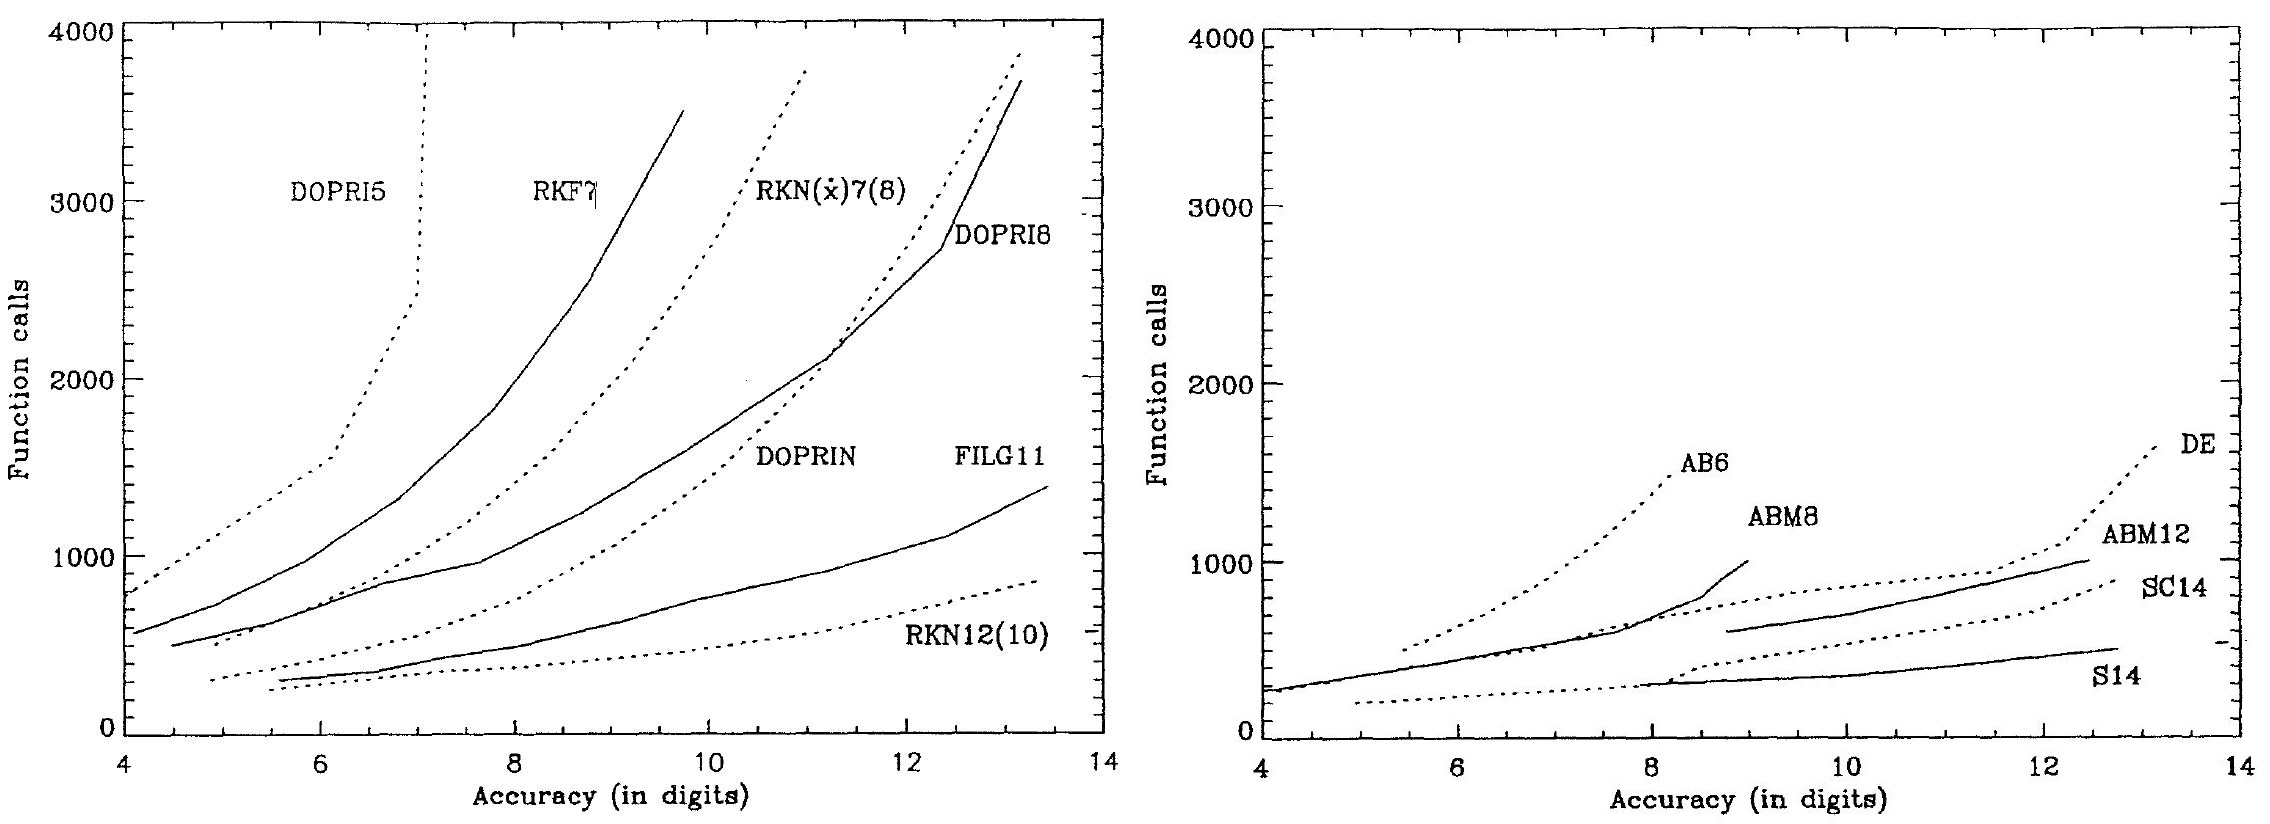
\includegraphics[width=1.0\textwidth]{figures/integrators/comp_single_multi_montenbruck1992.jpg}
\caption{Comparison of single-step (left) and multi-step (right) methods for an eccentricity of 0.1 \cite{montenbruck1992}.}
\label{fig:comp_single_multi_montenbruck1992}
\end{figure}
%
%\begin{figure}[!ht]
%\centering
%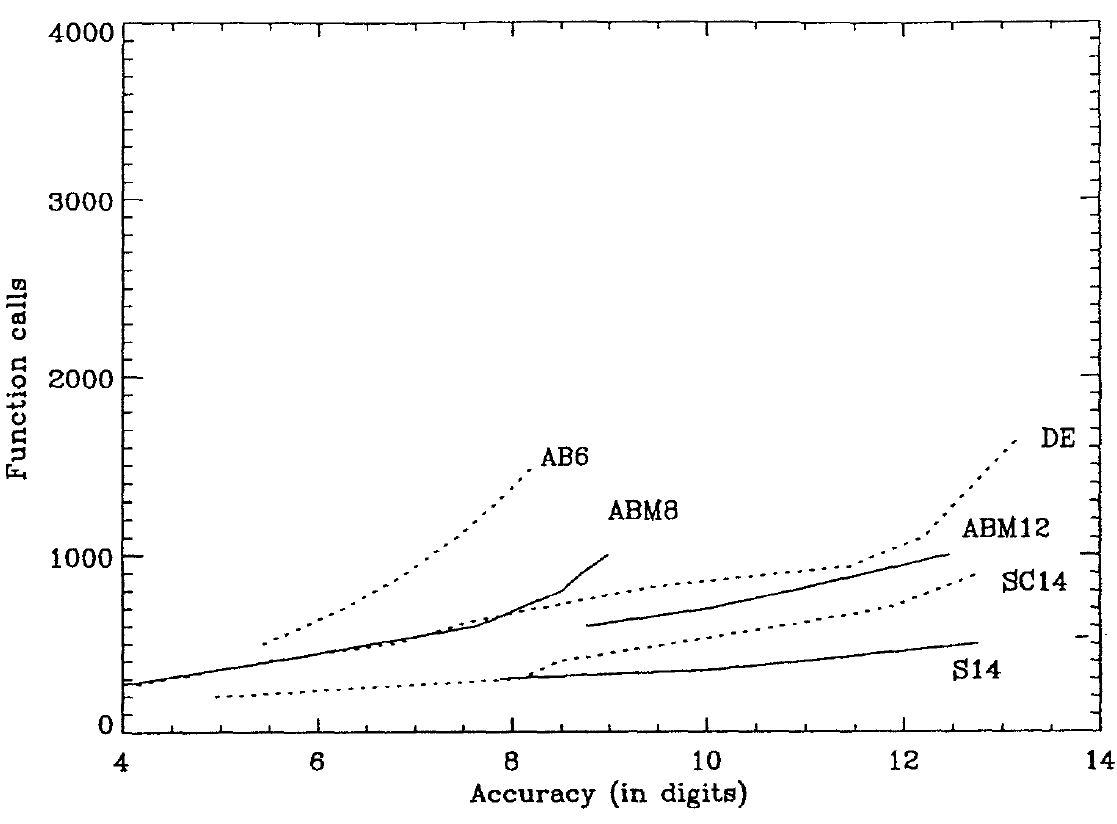
\includegraphics[width=0.5\textwidth]{figures/integrators/comp_multi_montenbruck1992.jpg}
%\caption{Comparison of multi-step methods for an eccentricity of 0.1 \cite{montenbruck1992}}
%\label{fig:comp_multi_montenbruck1992}
%\end{figure}





\section{Chosen methods}
\label{sec:intchosmeth}
For the integration method selection, it is beneficial to know which methods are used in industry and the scientific community (other universities included) and which methods have already been implemented within the Space department at the TU Delft. Some of the references used in \Cref{sec:difint,sec:inttechcomp} were already focussed on space missions but discussed a number of different methods. \Cref{subsec:intfreqmeth} elaborates on the implemented methods for space problems. The past TU Delft experience is discussed in \Cref{subsec:inther} and finally the methods are chosen in \Cref{subsec:chosintmeth}. 
%
%It is important to look at the experience that already exists within the department because that way it will be easier to learn from the people there, which is why the heritage will mainly decide the main methods. However, new developments or different theories from outside of the department should not be neglected, which is why these are also still considered as alternatives.

\subsection{Frequently used methods in related space problems}
\label{subsec:intfreqmeth}
\Cref{tab:intprevmeth} provides an overview of reference research and the used integrators. Should a reference discuss different methods, then the method that the author deems most suited for a space related mission will be cited. However, in some cases several methods are mentioned, since the detailed scope of the subjects was not set yet. In those cases, the proper application of the methods will be provided as well. 

\begin{table}[!ht]
\begin{center}
\caption{Previous integration methods used for trajectory and orbit (transfer) problems.}
\label{tab:intprevmeth}
\begin{tabular}{|l|l|p{5cm}|p{5cm}|}
\hline 
\textbf{Author} & \textbf{Year}		& \textbf{Subject} & \textbf{Method} \\ \hline \hline
Quinn et al. 	\cite{quinn1991} & 1991	& orbit propagation & St\"{o}rmer (so without Cowell implicit correction)  \\ \hline
Montenbruck \cite{montenbruck1992} & 1992 		& orbital motion (very low and very high elliptic orbits) & \ac{RKN12} (if \acs{EoM} $\neq f(V)$) else \ac{SG}  \\ \hline
Van der Houwen et al. 		\cite{houwen1998} & 1998 & high-precision orbit computations &  SC  \\ \hline
Gonz\'{a}lez et al. \cite{gonzalez2000} & 2000 & long-term satellite orbit prediction &  high-order RKN \\ \hline
Berry \cite{berry2004} &	2004	& space surveillance &  SC \\ \hline
Scott and Martini \cite{scott2008high} & 2008 & orbital motion, planetocentric and heliocentric trajectories & RKF89 and \ac{TSI}   \\ \hline
 		
% 		&  &   \\ \hline
\end{tabular}
\end{center}
\end{table}

\nomenclature[Ra3]{$V$}{Velocity\nomunit{m/s}}

%St\"{o}rmer-Cowell

%Unfortunately, often in literature, it is simply mentioned that an integration was performed, but then they fail to mention which method it was. 

A completely different category of integrators is the symplectic integration methods. These are used in orbit mechanics when dealing with a pure Hamiltonian system \cite{hofsteenge2013} and in the case of very long-term orbit integrations. However, since they deal with such a specific problem they are not considered useful for this thesis problem. %Widsom-Holman (1991) is often used

\subsection{TU Delft integration heritage}
\label{subsec:inther}
For the selection of the integration method, it is important to understand what has been done by previous master students and researchers at the Space department of the TU Delft. Because, information that already exists can be accessed more easily and it is also important to determine where improvements still have to be made. An overview of the different integrators used for research similar to the proposed thesis research is presented in \Cref{tab:intprevmethtu}.


\begin{table}[!ht]
\begin{center}
\caption{Previous integration methods used within the Space department.}
\label{tab:intprevmethtu}
\begin{tabular}{|l|l|p{5cm}|p{5cm}|}
\hline 
\textbf{Author} & \textbf{Year}		& \textbf{Subject} & \textbf{Method} \\ \hline \hline
%Van Kints \cite{noomen2013int} & 2005 & long-term stability of \ac{GEO} graveyard orbits & \ac{SC14} \\ \hline
Pagano \cite{pagano2010global} & 2010 & launch trajectories & \ac{RKF45} \\ \hline
R\"{o}mgens et al. \cite{romgens2011verified} & 2011 & satellite trajectories and collision avoidance & \ac{TSI} \\ \hline
Gondelach \cite{gondelach2012} & 2012 & low-thrust trajectories & \ac{RK4} \\ \hline
Vandamme \cite{vandamme2012assisted} & 2012 & launch trajectories & \ac{RK4} \\ \hline
Van Kesteren \cite{kesteren2013air} & 2013 & launch trajectories & \ac{RK4} \\ \hline
Hofsteenge \cite{hofsteenge2013} & 2013 & long-term propagation of space debris & DOPRI8 (similar to DOPRIN)\\ \hline
Gebbett \cite{gebbett2014multi} & 2014 & low-thrust trajectories & Adams-Moulton \\ \hline 
Boudestijn \cite{boudestijn2014} & 2014 & low-thrust trajectories & \ac{RK4}, RKF78 and Haun's method (extension of Euler)(best) \\ \hline
Gomez \cite{gomez2015optimization} & 2015 & low-thrust trajectories & Haun's method, \ac{ABM4} and \ac{RKF45} (best) \\ \hline
Miranda \cite{miranda2015} & 2015 & hybrid rockets  & \ac{RK4} \\ \hline  
    		
% 		&  &   \\ \hline
\end{tabular}
\end{center}
\end{table}

It is interesting to see that even though \ac{RK4} is not very accurate for large problems, it is still the preferred method for many master theses. 

%Within the space department, integration work has been performed by Van Kints in 2005 \cite{noomen2013int} (with \ac{SC14} performing best with Cartesian coordinates), Gondelach in 2012 \cite{gondelach2012} (using \ac{RK4}) and Hofsteenge in 2013 \cite{hofsteenge2013} (recommends DOPRI8, which is similar to DOPRIN). Although most methods used here are quite different, it is still important to understand which knowledge exists in the department. Research has also been performed on the \ac{TSI} by R\"{o}mgens et al. in 2011 \cite{romgens2011verified}.

\subsection{Chosen methods}
\label{subsec:chosintmeth}
Based on the reference research and the TU Delft heritage it has been decided to include \ac{RK4}, RKF (any order) and \ac{TSI} in the trade-off.
To provide flexibility in deciding on the final thesis topic, two different integration methods will be chosen. Then in \Cref{ch:findef} it will be determined whether to focus on two different integration methods or simply choose one. The decision of which methods to use will be based on the heritage, reference research, problem type (here launch and space trajectories), accuracy, speed, easy implementation and novelty. Also, the more resent the research the more relevant it is deemed to be. The trade-off is visualised using \Cref{tab:int_trade_off}. Every criterion is assigned a weight depending on how important the criterion is. Then the different methods are either green (1), yellow (0.5) or red (0) for every criterion. This results in a final score. 


\begin{table}[!ht]
\begin{center}
\caption{Optimiser trade-off table.}
\label{tab:int_trade_off}
\begin{tabular}{|l||l|l|l|l|l|l|l||l|}
\hline 
 &	\textbf{Heritage} & \textbf{Ref. research} & \textbf{Trajectories} & \textbf{Accuracy} & \textbf{Speed} & \textbf{Impl.} & \textbf{Novelty} & \textbf{Score}\\ \hline 
\textit{Weight} & \textit{4} & \textit{4} & \textit{5} & \textit{4} & \textit{3}  & \textit{2} & \textit{5} & \\ \hline \hline
\textbf{\ac{RK4}} & \cellcolor{green} & \cellcolor{red} & \cellcolor{green} & \cellcolor{red} &  \cellcolor{yellow}  & \cellcolor{green} & \cellcolor{red} & 12.5 \\ \hline
\textbf{RKF} & \cellcolor{green} & \cellcolor{yellow} & \cellcolor{green} & \cellcolor{yellow} & \cellcolor{yellow}  & \cellcolor{green} & \cellcolor{red} &  16.5 \\ \hline
\textbf{\ac{TSI}} & \cellcolor{yellow} & \cellcolor{yellow} & \cellcolor{yellow} & \cellcolor{green} & \cellcolor{green}  & \cellcolor{red} & \cellcolor{green} & 18.5  \\ \hline


\end{tabular}
\end{center}
\end{table}

From the trade-off table it is clear that \ac{TSI} shows potential for trajectories. However, as determined from the reference research and the TU Delft heritage, \ac{TSI} has not yet been used for launch trajectory integrations specifically. In \cite{scott2008high} \ac{TSI} was compared to RKF89 because the used program (SNAP) had this last integration method already incorporated. For an \ac{s/c} spiralling out of the Earth's gravity field, the cpu time required to integrate the problem with \ac{TSI} was found to be at least 19 times less than the time required to perform the same integration using RKF89. \ac{TSI} also proved to be more accurate for most cases.\\
RKF89 is a higher-order Runge-Kutta-Fehlberg method based on the original \ac{RKF45}. Both Pagano and Gomez used this original formulation of the \ac{RKF45} method. Boudestijn used a 7$^{th}$ order version of this method. \Cref{tab:int_trade_off} shwos that in this case it is also interesting to compare \ac{TSI} and RKF. Based on the fact that previous students have used \ac{RKF45} for both launch trajectories and (low-thrust) space trajectories (\cite{pagano2010global,gomez2015optimization}) this method will also be used for the integration of this thesis problem as well as \ac{TSI}. These two methods can then be compared to each other. \\
To gain a better understanding of \ac{TSI}, the implementation of this method will be discussed in \Cref{sec:imptsi}. \ac{RKF45} was originally based on \ac{RK4} and was described by Fehlberg in 1969 \cite{fehlberg1969}. Because it is based on \ac{RK4}, this method will be described in \Cref{sec:impothmeth}. Initially, \ac{RK4} can also be used to test the program. Later, both \ac{RKF45} and \ac{TSI} can be implemented and compared. The decision on whether to use different integration methods or just one of these will be made in the final topic trade-off in \Cref{ch:findef}.

%As mentioned in \Cref{ch:oversub} \ac{TSI} was already considered for the main integration method. This was done on the advice of the TU Delft supervisors mainly because no research has been done in the field of launch trajectories using this method. It would therefore be very interesting to use this method in such an application and compare it to other methods. However, at this point the focus will be on the optimisation and therefore the use of \ac{TSI} has become a secondary objective. This means that initially a simpler integration method will be used to model the trajectories and should time permit \ac{TSI} will be implemented. In \cite{scott2008high} \ac{TSI} was compared to \ac{RKF45} because the used program (SNAP) had this last integration method already incorporated. For an \ac{s/c} spiralling out of the Earth's gravity field, the cpu time required to integrate the problem with \ac{TSI} was found to be at least 19 times less than the time required to perform the same integration using \ac{RKF45}, which means that eventually it will be useful to try and use \ac{TSI} for the thesis problem as well. Therefore, the workings of \ac{TSI} are explained in \Cref{sec:imptsi}. However, by recommendation of the TU Delft supervisors, a simple initial integration method will suffice and can then later be compared to \ac{TSI} should time allow. Therefore, it will be best to start with the simplest integration method, the work-horse of the integration methods: \ac{RK4}. This is why this method will be discussed in more detail in \Cref{sec:impothmeth}. 

%Given the research performed in \cite{scott2008high} and the fact that SNAP already incorporates \ac{RKF45}, this method can be used initially. Should it however not be possible to use SNAP, a different program will have to be written. 

%Should time allow it though, it would be nice to also compare it to a more similar method to \ac{TSI}. Considering the different methods mentioned in \Cref{subsec:inther} the choice of similar reference method also highly depends on the methods mentioned in \Cref{subsec:intfreqmeth}. Therefore, at this point the best comparison method considered is \acl{SC14}. This is because \ac{SC14} has similar advantages and disadvantages to \ac{TSI} and it would therefore be interesting to determine which of the two methods produces the better results in case of the thesis problem. This will be taken into account for the secondary objective of the thesis.

% Still however taking into account the existing experience of the space department.

% St\"{o}rmer-Cowell

\section{Implementation of \ac{TSI}}
\label{sec:imptsi}
\ac{TSI} has been used to solve ordinary differential equations since the early 1960s \cite{scott2008high}. However, the first modern implementation of \ac{TSI} in a space trajectory problem was provided by Montenbruck in 1992 \cite{montenbruck1992numerical,scott2010high}. In 2008 Scott and Martini were able to implement this \ac{TSI} method into the SNAP trajectory propagator \cite{scott2008high} which is the implementation that will be used during this explanation. The method used is described in \Cref{subsec:worktsi} and possible improvements on the method are mentioned in \Cref{subsec:vartsi}. 

\subsection{Workings of \ac{TSI}}
\label{subsec:worktsi}
In \cite{scott2008high} an example situation is used to describe the \ac{TSI} method: the thrust-less motion around a central body. For consistency the same example and formulation will be used. The state vector is represented by $\mathbf{X}$ with the corresponding vector for the initial conditions $\mathbf{X}_{0}$. Each of the variables can at any point be represented by $x_{n}\left(t\right)$ and thus the Taylor series expansion for an order $K \in \mathbb{R}$ (chosen by the user) can be written as shown by \Cref{eq:general_taylor} with $n=1,\dots,7$ in this case (7 variables: three position, three velocity and one mass) and $T_{n,K}$ is the truncation error for the $n^{th}$ variable using K terms. 

\nomenclature[Ra7]{$\mathbf{X}$}{State vector \nomunit{-}}
\nomenclature[Ra6]{$x_{n}$}{n$^{th}$ variable \nomunit{-}}
\nomenclature[Ra2]{$T_{n,k}$}{Truncation error \nomunit{-}}


\begin{equation} \label{eq:general_taylor}
x_{n}\left(t\right)=\displaystyle\sum_{k=0}^{K}\dfrac{x_{n}^{\left(k\right)}\left(t_{0}\right)}{k!}\left(t-t_{0}\right)^{k} \quad + \quad	T_{n,K}
\end{equation}

This particular \ac{TSI} method uses recurrence relations to determine the $k^{th}$ order derivatives and only requires the first derivatives shown in \Cref{eq:first_deri} for the 7 variables and two newly introduced variables to ease the use of the recurrence relations. Here $GM$ represents the standard gravitational parameter (also known as $\mu$).

\begin{equation} \label{eq:first_deri}
\begin{split}
x_{1}'&=x_{4}\\
x_{2}'&=x_{5}\\
x_{3}'&=x_{6}\\
x_{4}'&=-GM\dfrac{x_{1}}{\left(x_{1}^{2}+x_{2}^{2}+x_{3}^{2} \right)^{3/2}}=-GM\dfrac{x_{1}}{x_{9}} \quad \text{with} \quad x_{9}=x_{8}^{3/2} \quad \text{and} \quad x_{8}=x_{1}^{2}+x_{2}^{2}+x_{3}^{2}\\
x_{5}'&=-GM\dfrac{x_{2}}{\left(x_{1}^{2}+x_{2}^{2}+x_{3}^{2} \right)^{3/2}}=-GM\dfrac{x_{1}}{x_{9}}\\
x_{6}'&=-GM\dfrac{x_{3}}{\left(x_{1}^{2}+x_{2}^{2}+x_{3}^{2} \right)^{3/2}}=-GM\dfrac{x_{1}}{x_{9}}\\
x_{7}'&=0\\
x_{8}'&=2x_{1}x_{4}+2x_{2}x_{5}+2x_{3}x_{6}\\
x_{9}'&=\dfrac{3}{2}\dfrac{x_{9}x_{8}'}{x_{8}}\\
\end{split}
\end{equation}

The general recurrence relations for products ($w\left(t\right)=f\left(t\right)g\left(t\right)$) and quotients ($w\left(t\right)=\dfrac{f\left(t\right)}{g\left(t\right)}$) that are required are provided in \Cref{eq:rec_rel} respectively.

\begin{equation} \label{eq:rec_rel}
\begin{split}
&\text{For products} \quad W\left(k\right)=\displaystyle\sum_{j=0}^{k}F\left(j\right)G\left(k-j\right)\\
&\text{For quotients} \quad W\left(k\right)=\dfrac{1}{g\left(t_{0}\right)}\left[F\left(k\right)-\displaystyle\sum_{j=1}^{k} G\left(j\right)W\left(k-j\right)\right]\\
& Both \ with \quad W\left(k\right)=\dfrac{w^{\left(k\right)}\left(t_{0}\right)}{k!}, \quad F\left(j\right)=\dfrac{f^{\left(j\right)}\left(t_{0}\right)}{j!} \quad \text{and} \quad G\left(k-j\right)=\dfrac{g^{\left(k-j\right)}\left(t_{0}\right)}{\left(k-j\right)!}\\
\end{split}
\end{equation}


Now let $u_{n}^{\left(k-1\right)}=x_{n}^{k}$ for $k=1,\dots,K$, then $\dfrac{u_{n}^{\left(k-1\right)}}{\left(k-1\right)!}=\dfrac{x_{n}^{k}}{\left(k-1\right)!}$, and also $\dfrac{x_{n}^{k}}{k!}=X_{n}\left(k\right)$. Combining this results in \Cref{eq:def_u}.

\begin{equation} \label{eq:def_u}
U_{n}\left(k-1\right)=kX_{n}\left(k\right)\Rightarrow X_{n}\left(k\right)=\dfrac{U_{n}\left(k-1\right)}{k}
\end{equation}
 
Then also introducing $w_{4}=\dfrac{x_{1}}{x_{9}}$, $w_{5}=\dfrac{x_{2}}{x_{9}}$, $w_{6}=\dfrac{x_{3}}{x_{9}}$, $w_{8,1}=x_{1}x_{4}$, $w_{8,2}=x_{2}x_{5}$, $w_{8,3}=x_{3}x_{6}$ and $w_{9}=\dfrac{x_{9}u_{8}}{x_{8}}$, the equations presented in \Cref{eq:first_deri} can be rewritten to arrive at the recurrence relations using the provided definitions. These relations are presented in \Cref{eq:full_rec_rel}. 

%\begin{equation} \label{eq:full_rec_rel}
%\begin{split}
%U_{1}\left(k\right)&=X_{4}\left(k\right)=\dfrac{U_{4}\left(k-1\right)}{k}\\
%U_{2}\left(k\right)&=X_{5}\left(k\right)=\dfrac{U_{5}\left(k-1\right)}{k}\\
%U_{3}\left(k\right)&=X_{6}\left(k\right)=\dfrac{U_{5}\left(k-1\right)}{k}\\
%U_{4}\left(k\right)&=-GMW_{4}\left(k\right)\\
%U_{5}\left(k\right)&=-GMW_{5}\left(k\right)\\
%U_{6}\left(k\right)&=-GMW_{6}\left(k\right)\\
%U_{7}\left(k\right)&=0\\
%U_{8}\left(k\right)&=2W_{8,1}\left(k\right)+2W_{8,2}\left(k\right)+2W_{8,3}\left(k\right)\\
%U_{9}\left(k\right)&=\dfrac{3}{2}W_{9}\left(k\right)\\
%\end{split}
%\end{equation}


\begin{align} \label{eq:full_rec_rel}
\begin{split} 
U_{1}\left(k\right)&=X_{4}\left(k\right)=\dfrac{U_{4}\left(k-1\right)}{k}\\
U_{2}\left(k\right)&=X_{5}\left(k\right)=\dfrac{U_{5}\left(k-1\right)}{k}\\
U_{3}\left(k\right)&=X_{6}\left(k\right)=\dfrac{U_{5}\left(k-1\right)}{k}
\end{split} 
&
\begin{split}
U_{4}\left(k\right)&=-GMW_{4}\left(k\right)\\
U_{5}\left(k\right)&=-GMW_{5}\left(k\right)\\
U_{6}\left(k\right)&=-GMW_{6}\left(k\right)
\end{split}
&
\begin{split}
U_{7}\left(k\right)&=0\\
U_{8}\left(k\right)&=2W_{8,1}\left(k\right)+2W_{8,2}\left(k\right)+2W_{8,3}\left(k\right)\\
U_{9}\left(k\right)&=\dfrac{3}{2}W_{9}\left(k\right)
\end{split}
\end{align}

Where the expressions for $W_{4}\left(k\right)$, $W_{5}\left(k\right)$, $W_{6}\left(k\right)$, $W_{8,1}\left(k\right)$, $W_{8,2}\left(k\right)$, $W_{8,3}\left(k\right)$ and $W_{9}\left(k\right)$ are shown in \Cref{eq:express_W}.

\begin{equation} \label{eq:express_W}
\begin{split}
W_{4}\left(k\right)&=\dfrac{1}{x_{9}}\left[X_{1}\left(k\right)-\displaystyle\sum_{j=1}^{k}X_{9}\left(j\right)W_{4}\left(k-j\right)\right]=\dfrac{1}{x_{9}}\left[\dfrac{U_{1}\left(k-1\right)}{k}-\displaystyle\sum_{j=1}^{k}\dfrac{U_{9}\left(j-1\right)}{k}W_{4}\left(k-j\right)\right]\\
W_{5}\left(k\right)&=\dfrac{1}{x_{9}}\left[X_{2}\left(k\right)-\displaystyle\sum_{j=1}^{k}X_{9}\left(j\right)W_{5}\left(k-j\right)\right]=\dfrac{1}{x_{9}}\left[\dfrac{U_{2}\left(k-1\right)}{k}-\displaystyle\sum_{j=1}^{k}\dfrac{U_{9}\left(j-1\right)}{k}W_{5}\left(k-j\right)\right]\\
W_{6}\left(k\right)&=\dfrac{1}{x_{9}}\left[X_{3}\left(k\right)-\displaystyle\sum_{j=1}^{k}X_{9}\left(j\right)W_{6}\left(k-j\right)\right]=\dfrac{1}{x_{9}}\left[\dfrac{U_{3}\left(k-1\right)}{k}-\displaystyle\sum_{j=1}^{k}\dfrac{U_{9}\left(j-1\right)}{k}W_{6}\left(k-j\right)\right]\\
W_{8,1}\left(k\right)&=\displaystyle\sum_{j=0}^{k}X_{1}\left(j\right)X_{4}\left(k-j\right)=x_{1}\dfrac{U_{4}\left(k-1\right)}{k}+x_{4}\dfrac{U_{1}\left(k-1\right)}{k}+\displaystyle\sum_{j=1}^{k-1}\dfrac{U_{1}\left(j-1\right)}{j}\dfrac{U_{4}\left(k-j-1\right)}{k-j}\\
W_{8,2}\left(k\right)&=\displaystyle\sum_{j=0}^{k}X_{2}\left(j\right)X_{5}\left(k-j\right)=x_{2}\dfrac{U_{5}\left(k-1\right)}{k}+x_{5}\dfrac{U_{2}\left(k-1\right)}{k}+\displaystyle\sum_{j=1}^{k-1}\dfrac{U_{2}\left(j-1\right)}{j}\dfrac{U_{5}\left(k-j-1\right)}{k-j}\\
W_{8,3}\left(k\right)&=\displaystyle\sum_{j=0}^{k}X_{3}\left(j\right)X_{6}\left(k-j\right)=x_{3}\dfrac{U_{6}\left(k-1\right)}{k}+x_{6}\dfrac{U_{3}\left(k-1\right)}{k}+\displaystyle\sum_{j=1}^{k-1}\dfrac{U_{3}\left(j-1\right)}{j}\dfrac{U_{6}\left(k-j-1\right)}{k-j}\\
W_{9}\left(k\right)&=\dfrac{1}{x_{8}}\left[\displaystyle\sum_{j=0}^{k}X_{9}\left(j\right)U_{8}\left(k-j\right)-\displaystyle\sum_{j=1}^{k}X_{8}\left(j\right)W_{9}\left(k-j\right)\right]\\
&=\dfrac{1}{x_{8}}\left[\displaystyle\sum_{j=0}^{k}\dfrac{U_{9}\left(j-1\right)}{j}U_{8}\left(k-j\right)-\displaystyle\sum_{j=1}^{k}\dfrac{U_{8}\left(j-1\right)}{j}W_{9}\left(k-j\right)\right]\\
\end{split}
\end{equation}

With the Taylor series coefficients now defined as provided in \Cref{eq:def_u}, \Cref{eq:general_taylor} can be used to determine the parameter values at time $t$ (or $t_{1}$) for the known previous parameter values at time $t_{0}$. The same can then be done to determine the values at $t_{2}$ using the parameter values at $t_{1}$, etc. In its simplest form, a constant step-size $h$ (defined as $t-t_{0}$) is taken which determines the next $t$.


\subsection{Variations of \ac{TSI}}
\label{subsec:vartsi}
Many of the different aspects of \ac{TSI} can be varied upon: the manner in which the truncation error is estimated, the order $K$ until which the series is evaluated, the use of a variational step-size and the method of determining the next step size.\\

As mentioned before $K$ should be chosen by the user, however in \cite{scott2008high} it is mentioned that the maximum number of series terms cannot exceed 30 using this particular method. 

When considering the variable step-size, \cite{scott2008high} uses two different methods to determine the next step size. The first method is using \Cref{eq:stand_stsi}, where $\eta$ is the chosen step multiplication factor and has to be smaller than 1, $h$ is the current step-size, $\tau$ is the chosen local error tolerance (or preferred accuracy), $e_{max}$ is the estimate of maximum truncation error and $M$ is the order of the maximum truncation error estimate which follows from the maximum number of series terms.

\nomenclature[G3]{$\eta$}{Step multiplication factor \nomunit{-}}
%\nomenclature{$h$}{Current step-size \nomunit{s}}
\nomenclature[G6]{$\tau$}{Local error tolerance \nomunit{-}}
\nomenclature[R1]{$e_{max}$}{Estimate of maximum truncation error \nomunit{-}}
\nomenclature[R8]{$M$}{Order of the maximum truncation error estimate \nomunit{-}}

%Note to self: can \eta be chosen by the user at random?

\begin{equation} \label{eq:stand_stsi}
h_{next}=\eta h\left(\dfrac{\tau}{e_{max}}\right)^{\frac{1}{M}}
\end{equation} 

In this case $e_{max}$ is determined through \Cref{eq:emax}. The maximum estimated truncation error over all variables $n$ is chosen.

\begin{equation} \label{eq:emax}
e_{max}=Max_{n}\left[\begin{vmatrix}
X_{n}\left(K-1\right)
\end{vmatrix} h^{K-1}+ \begin{vmatrix}
X_{n}\left(K\right)
\end{vmatrix} h^{K}\right]
\end{equation}

Another method mentioned in the same paper is to directly use the local error tolerance $\tau$ to determine the next step size. This method assures that the step-size is small enough that all variables satisfy the error condition directly. The step-size is determined using a so-called fixed-point iteration performed using \Cref{eq:fix_point_it}. The initial step-size $h_{1}$ can be chosen to be the current step-size $h$ as an easy estimate. Then the iteration is performed over $l$ until a certain required convergence is reached.

\begin{equation} \label{eq:fix_point_it}
h_{l+1}=exp\left(\dfrac{1}{K-1}ln\left[\dfrac{\tau}{\begin{vmatrix}
X_{n}\left(K-1\right)
\end{vmatrix}+h_{l}\begin{vmatrix}
X_{n}\left(K\right)
\end{vmatrix}}\right]\right)
\end{equation}

Again this is done for all variables and the smallest required step-size is chosen. This is then used to determine the next step-size through $h_{next}=\eta h_{chosen}$. Scott and Martini preferred this second method over the first mentioned method of determining the next step-size because the first method requires previous step information ($e_{max}$), nonetheless the performance of both methods was very similar \cite{scott2008high}.

Finally, there are several techniques to estimate the (local) truncation error that results from every series evaluation. Simply put $e_{max}$ is the estimation of the maximum value that $T_{n,K}$ can take. One example of how to determine this estimate was already shown by \Cref{eq:emax}. Another approach would be to calculate the estimate from the K+1 term in the series, however, this is discouraged in \cite{scott2008high} where it is said that it would require an extra computation and is not a reliable error estimate.

%Note to self: I do not understand how you can determine the truncation error if you do not know the exact solution. And if you do know the exact solution there is no use in using a numerical approximation right?!....



\section{Implementation of \ac{RK4}}
\label{sec:impothmeth}
\ac{RK4} is known as the work-horse of engineering problems when it comes to the integration of functions. It is a slightly more complicated form of the Euler and Mid-point methods. In this case four points/state vectors are used to determine the next parameter value(s). The exact workings of \ac{RK4} will be explained in \Cref{subsec:work_rk4} and other variations are discussed in \Cref{subsec:var_rk4}.



\subsection{Workings of \ac{RK4}}
\label{subsec:work_rk4}
\ac{RK4} is based on the formulation provided by \Cref{eq:integration} where in this case the increment function for \ac{RK4} is presented in \Cref{eq:rk4_increment}. The principle behind \ac{RK4} is well described by \cite{noomen2013int}. This method is a single-step, fixed step-size, explicit method and thus does not use any previous step information to determine the next step. Only the current parameter values are used to predict the next step as is visualised in \Cref{fig:rk4_noomen2013int}. In this figure it can also be seen that this method uses four derivative evaluations of the function to determine the next point indicated as $x\left(t_{0}+h\right)$. 


\begin{equation} \label{eq:rk4_increment}
\Phi_{RK4}=\dfrac{1}{6}\left(k_{1}+2k_{2}+2k_{3}+k_{4}\right)
\end{equation}


\begin{figure}[!ht]
\centering
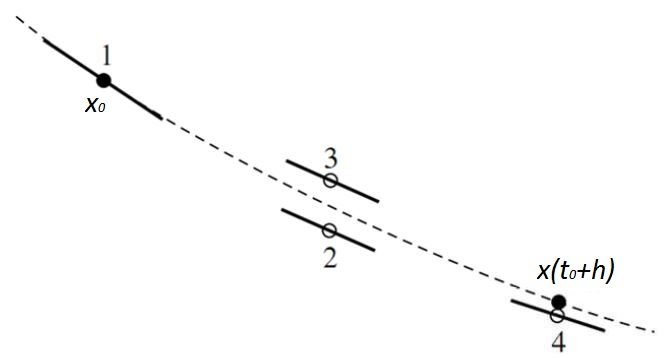
\includegraphics[width=0.3\textwidth]{figures/integrators/rk4_noomen2013int.jpg}
\caption{Principle of \ac{RK4} for a single parameter \cite{noomen2013int}.}
\label{fig:rk4_noomen2013int}
\end{figure}

First the time-derivative of the current point/state vector is taken and called $k_{1}$ as shown by \Cref{eq:k} (including the whole sequence). This is used to evaluate the local state vector halfway through the interval at $h/2$ from the current time and for a parameter value of $x_{0}+h\dfrac{k_{1}}{2}$ and is called $k_{2}$. This $k_{2}$ is then used instead of $k_{1}$ to perform the same evaluation as before, resulting in $k_{3}$. Finally, $k_{3}$ is used to evaluate the local state vector at the end of the interval resulting in $k_{4}$. These four derivative values are then added in a weighted fashion to produce the increment function as shown by \Cref{eq:rk4_increment}, which is in turn used to determine the next point/state vector (see \Cref{eq:integration}). 


\begin{equation} \label{eq:k}
\begin{split}
k_{1}&=f'\left(t_{0},x_{0}\right)\\
k_{2}&=f'\left(t_{0}+h/2,x_{0}+hk_{1}/2\right)\\
k_{3}&=f'\left(t_{0}+h/2,x_{0}+hk_{2}/2\right)\\
k_{4}&=f'\left(t_{0}+h,x_{0}+hk_{3}\right)\\
\end{split}
\end{equation}

In \Cref{eq:k} $f'$ depicts the evaluation of the derivative. It is also mentioned in \cite{noomen2013int} that performing this integration will result in a local truncation error that is $O\left(h^{5}\right)$. Therefore, \Cref{eq:integration} can be adapted to include the truncation error as depicted by \Cref{eq:trunc_int}.



\begin{equation} \label{eq:trunc_int}
\mathbf{x}(t_{0}+h)=\mathbf{x}_{0}+h\bm{\Phi}+\mathbf{T}
\end{equation}


\subsection{Methods based on \ac{RK4}}
\label{subsec:var_rk4}
The \ac{RK4} method is often seen as the classic method and has thus been expanded and varied upon substantially (also see \Cref{subsec:single}). There are three direct means in which to modify the method: the order (so number of intermediate points used to evaluate the final point), including the next estimation to improve the next parameter values (making it implicit) and the manner in which the step-size is chosen, which can even be done such that the method changes to a variable step-size method. Examples of implicit methods based on \ac{RK4} are DOPRIN and \ac{RKN12}, and an example of a method which is based on \ac{RK4} but uses a variable step-size is \ac{RKF45}. The \ac{RKF45} uses an estimate of the truncation error to determine the next step-size \cite{fehlberg1969}, similar to a variation of \ac{TSI}. This is accomplished by computing a fourth and fifth order Runge-Kutta and then using the difference between those two as an estimate for the truncation error. Then the step-size can be adjusted if required.








